\synctex=1
\documentclass[dvipdfmx,10pt, a4j]{jarticle}
%----------------------------------------------------------
%パッケージ読み込み
\usepackage{amsmath}
\usepackage{amssymb}
\usepackage{amsthm} %定理環境の拡張
\usepackage{ascmac}
\usepackage{bm}
\usepackage{cases}
\usepackage{comment} %非表示にするためのコメント
\usepackage{enumerate}
\usepackage{float} %画像をその場に表示.[h]の代わりに[H]
\usepackage{graphicx} % eps 形式の図版取り込みのため
\usepackage{mathrsfs}
\usepackage{url}
\usepackage[dvipdfmx]{hyperref}
\usepackage{color}
%----------------------------------------------------------

%----------------------------------------------------------
%命題関係の定義
\theoremstyle{definition}
\newtheorem{definition}{定義}[section]
\newtheorem{theorem}{定理}[section]
\newtheorem{proposition}[theorem]{命題}
\newtheorem{lemma}[theorem]{補題}
\newtheorem{col}[theorem]{系}
\newtheorem{example}{例}[section]
\newtheorem{remark}{注意}[section]
%----------------------------------------------------------

%タイトル・著者===================================================
\title{第9回 数理統計 レポート}
\author{小森 一輝}
%=================================================================

%本文開始=========================================================
\begin{document}

\maketitle

%カウンタ--------------------------------------------------
\setcounter{section}{2}
%\setcounter{subsection}{0}
%\setcounter{subsubsection}{0}
%\setcounter{theorem}{0}

%----------------------------------------------------------定義4.1
\noindent
\textbf{定義 4.1.} 多次元確率変数\\
$確率空間(\Omega, \mathscr{A}, P)において, 写像の組 \mathbb{X} = (X_1, X_2, \dots, X_n):\Omega \to \mathbb{R}^{n}が任意の集合\mathbf{B} \in \mathscr{B}^{n}に対して,$\\
\begin{align*}
    \mathbb{X}^{-1}(\mathscr{B}) = \{\omega \mid \mathbb{X}(\omega) \in \mathbf{B}\} \in \mathscr{A} \\
\end{align*}
$を満たすならば, \mathbb{X} はn \textbf{次元確率変数 (n dimensional random vraiable)} とよばれる.$\\
$ここで, \mathbf{B} = \prod_{i=1}^{n}B_i (=B_1 \times B_2 \times \cdots \times B_n), B_i \in \mathscr{B} (i = 1,2, \dots ,n)である.$\\

%----------------------------------------------------------定理4.1
\noindent
\textbf{定理 4.1.} $確率空間 (\Omega, \mathscr{A}, P) において, 写像の組 \mathbb{X} = (X_1, X_2, \dots, X_n):\Omega \to \mathbb{R}^{n}$
$がn次元確率変数であるための必要十分条件は, \mathbb{X} が,$
\begin{align*}
    \mathbb{X}^{-1} = \{\omega \mid \mathbb{X}(\omega) \leq x\} \in \mathscr{A} \qquad (x \in \mathbb{R}^{n}) \\
\end{align*}
を満たすことである.ここで,\\
\begin{align*}
    \{\omega \mid \mathbb{X}(\omega) \leq x\} = \{\omega \mid X_1(\omega) \leq x_1, X_2(\omega) \leq x_2, \dots , X_n(\omega) \leq x_n\} \\
\end{align*}
であり,\\
\begin{align*}
    I^{n} = \prod (- \infty, x_i] = (- \infty, x_1] \times (- \infty, x_2] \times \cdots \times (- \infty, x_n] \\
\end{align*}
である.\\

%----------------------------------------------------------定義4.2
\noindent
\textbf{定義 4.2.} 同時確率分布\\
$確率空間(\Omega, \mathscr{A}, P)における, n次元確率変数 \mathbb{X} = (X_1, X_2, \dots, X_n) に対して,$\\
\begin{align*}
    P_{\mathbb{X}}(\mathbf{B}) = P(\mathbb{X}^{-1}(\mathbf{B})) \qquad (\mathbf{B} \in \mathscr{B}^{n}) \\
\end{align*}
$によって定義される(\mathbb{R}^{n}, \mathscr{B}^{n})上の確率測度P_{\mathbb{X}}は \mathbb{X} の \textbf{同時確率分布 (joint probability distribution)}$
$とよばれる. このとき, \mathbb{X} は P_{\mathbb{X}}に従うといい, X \sim P_{\mathbb{X}} と記す.$\\

%----------------------------------------------------------定義4.3
\noindent
\textbf{定義 4.3.} 周辺確率分布\\
$確率空間 (\Omega, \mathscr{A}, P)における, n次元確率変数 \mathbb{X} = (X_1, X_2, \dots, X_n) に対して,$
$\mathbb{X}_{(p)} = (X_{i1}, X_{i2}, \dots , X_{ip}) (1 \leq p < n; 1 \leq i_1 \leq i_2 < \cdots < i_p \leq n)としたとき,$\\
\begin{align*}
    P_{\mathbb{X}_{(p)}}(\mathbf{B_{(p)}}) = P \left(\mathbb{X}_{(p)}^{-1}(\mathbf{B}_{(p)}) \right) \qquad (\mathbf{B}_{(p)} \in \mathscr{B}^{p})\\
\end{align*}
$によって定義される, (\mathbb{R}^{p}, \mathbb{B}^{p}) 上の確率測度 P_{\mathbb{X}} は \mathbb{X}_{(p)} の \textbf{周辺確率分布(marginal probability distribution)}$
$とよばれる. ここで, \mathbf{B}_{(p)} = \prod_{j=1}^{p}{B_{ij}}である.$\\

%----------------------------------------------------------定義4.4
\noindent
\textbf{定義 4.4.} 条件付き確率分布\\
$確率空間 (\Omega, \mathscr{A}, P)における n次元確率変数 \mathbb{X} = (X_1, X_2, \dots, X_n)を, \mathbb{X} = (\mathbb{X}_{(p)}, \mathbb{X}_{(q)})$
$と2つに分ける. ただし, 一般性を失うことなく,$\\
\begin{align*}
    \mathbb{X}_{(p)} = (X_{i1}, X_{i2}, \dots, X_{ip}),\; \mathbb{X}_{(q)} = (X_{j1}, X_{j2}, \dots, X_{jq})\\
\end{align*}
$であり, 添え字集合 I = (i_1, i_2, \dots, i_p), J = (j_1, j_2, \dots, j_q) に関して,$\\
\begin{align*}
    I \cup J = \{1,2, \dots, n\},& \qquad I \cap J = \phi\\
    1 \leq p < n,& \qquad q = n - p\\
    1 \leq i_1 < i_2 < \cdots < i_p \leq n,& \qquad 1 \leq j_1 < j_2 < \cdots < j_q \leq n\\
\end{align*}
$が成り立っているとする. このとき,$\\
\begin{align*}
    P_{(\mathbb{X}_{(p)} \mid \mathbb{X}_{(q)})}(\mathbf{B}_{(p)} \mid x_{(q)}) =
        \begin{cases}
            \frac{P\left(\mathbb{X}^{-1} (\mathbf{B}_{(p)} \times \{x(q)\}\right)}{p(\mathbb{X}_{(q)}^{-1}(\{x_{(q)}\}))} \qquad &\left(p(\mathbb{X}_{(q)}^{-1}(\{x_{(q)}\})) > 0 \right)\\
            0 \qquad &\left(p(\mathbb{X}_{(q)}^{-1}(\{x_{(q)}\})) = 0 \right)\\
        \end{cases}\\
\end{align*}
$によって定義される(\mathbb{R}^{p}, \mathscr{B}^{p}) 上の確率測度 P_{\mathbb{X}_{(p)} \mid \mathbb{X}_{(q)}} を \mathbb{X}_{(q)} = x_{(q)} が与えられたときの$
$\mathbb{X}_{(p)} の\textbf{条件付き確率分布(conditional probability distribution)} とよぶ.$\\
$ここで\mathbf{B}_{(p)} = \prod_{k=1}^{p} B_{ik} \in \mathscr{B}^{p} であり, \{x_{q}\} = \prod_{k=1}^{q} \{x_{jk}\}である.$\\

%----------------------------------------------------------定義4.5
\noindent
\textbf{定義 4.5.} 同時確率分布\\
$確率空間 (\Omega, \mathscr{A}, P) における n次元確率変数 \mathbb{X}に対して,$\\
\begin{align*}
    F_{\mathbb{X}}(x) = P_{\mathbb{X}}\left(\prod_{i-1}^{n} (- \infty, x_i] \right) = P(\mathbb{X} \leq x) \qquad (x \in \mathbb{R}^{n})\\
\end{align*}
$で定義される \mathbb{R}^{n} 上の実数関数 F_{\mathbb{X}}を\mathbb{X}の \textbf{同時分布関数 (joint distribution function)} とよぶ.$\\

%----------------------------------------------------------定義4.6
\noindent
\textbf{定義 4.6.} 周辺分布関数\\
$確率空間 (\Omega, \mathscr{A}, P) における n次元確率変数 \mathbb{X} = (X_1, X_2, \dots, X_n) に対して,$
$n次元確率変数 \mathbb{X}_{(p)} = (X_{i_1}, X_{i_2}, \dots, X_{i_p}) (1 \leq p < n;\; 1 \leq i_1 < i_2 < \cdots < i_p \leq n) としたとき,$
\begin{align*}
    F_{\mathbb{X}_{(p)}}(x_{(p)} &= F_{\mathbb{X}}(\infty, \dots , \infty, x_{i_1}, \infty, \dots , \infty, x_{i_p}, \infty, \dots , \infty)\\
    &= P(X_{i_1} \leq x_{i_1}, X_{i_2} \leq x_{i_2}, \dots , X_{i_p} \leq x_{i_p})\\
    &= P(X_{p} \leq x_{p})\\
\end{align*}
$を \mathbb{X}_{(p)} の \textbf{周辺分布関数 (marginal distribution function)} とよぶ.$\\

%----------------------------------------------------------定義4.7
\noindent
\textbf{定義 4.7.} 条件付き分布関数\\
$確率空間 (\Omega, \mathscr{A}, P) における n次元確率変数 \mathbb{X} = (X_1, X_2, \dots, X_n) を定義4.4 と$
$同時 \mathbb{X} = (\mathbb{X}_{(p)}, \mathbb{X}_{(q)}) と2つに分ける. このとき,$\\
\begin{align*}
    F_{\mathbb{X}_{(p)} \mid \mathbb{X}_{(q)}} = 
    \begin{cases}
        \frac{P(\mathbb{X}_{(p)}) \leq x_{(p)}, \mathbb{X}_{(q)} = x_{(q)}}{P(\mathbb{X}_{(q)} = x_{(q)})}& \qquad \left(P \left( \mathbb{X}_{(q)} = x_{(q)} \right) > 0 \right)\\
        0& \qquad \left(P \left( \mathbb{X}_{(q)} = x_{(q)} \right) = 0 \right)\\
    \end{cases}\\
\end{align*}
$を \mathbb{X}_{(q)} = x_{(q)} を与えられたときの \mathbb{X}_{(p)} の \textbf{条件付き分布関数 (conditional distribution function)} とよぶ.$\\

%----------------------------------------------------------定義4.8
\noindent
\textbf{定義 4.8.} n次元離散型確率変数\\
$n次元確率変数 \mathbb{X} = (X_1, X_2, \dots, X_n) に対して, ある集合$\\
\begin{align*}
    E = \{x_k = (x_{k1}, x_{k2}, \dots , x_{kn}) \mid k=1,2, \dots \} \subset \mathbb{R}\\
\end{align*}
$が存在し, P(\mathbb{X} \in E) = 1 を満たすとき, \mathbb{X} を \textbf{n次元離散型確率変数 (n dimensional discrete random vraiable)} とよぶ.$\\

$\mathbb{X} が n次元離散型確率変数のとき, x_k \in E(k=1,2, \dots ) に対して, p_k = P_{\mathbb{X}}(\{x_k\}) とすれば,$\\
\begin{align*}
    \sum_{k=1}^{\infty}p_k = 1, \qquad F_{\mathbb{X}}(x) = \sum_{x_i \leq x}p_k\\
\end{align*}
が成り立つ.\\

%----------------------------------------------------------定義4.9
\noindent
\textbf{定義 4.9.} 同時確率関数\\
$n次元離散型確率変数 \mathbb{X} = (X_1, X_2, \dots, X_n) に対して, \mathbb{R}^{n} 上の実数値関数$\\
\begin{align*}
    f_{\mathbb{X}}(x) = 
    \begin{cases}
        p_k = P(\mathbb{X} = x_i) \qquad &(x = x_i \in E(k=1,2, \dots))\\
        0 \qquad &(x \notin E)\\
    \end{cases}\\
\end{align*}
$を \mathbb{X} の \textbf{同時確率関数 (joint probability function)} とよぶ. ここで, E= \{x_k = \{x_{k1}, x_{k2}, \dots , x_{kn}\} \mid k=1,2, \dots \} \subset \mathbb{R}^{n}である.$\\

%----------------------------------------------------------定義4.10
\noindent
\textbf{定義 4.10.} 周辺確率関数\\
$n次元離散型確率変数 \mathbb{X} = (X_1, X_2, \dots, X_n) を定義4.4と同時に \mathbb{X} = (\mathbb{X}_{(p)}, \mathbb{X}_{(q)})と2つに分ける. このとき,$\\
\begin{align*}
    f_{\mathbb{X}_{(p)}}(x_{(p)}) = \sum_{j1 = 1}^{\infty} \sum_{j2 = 1}^{\infty} \cdots \sum_{jq = 1}^{\infty} f_{\mathbb{X}}(x) = P\left(\mathbb{X}_{(p)} = x_{(p)} \right)\\
\end{align*}
$を \mathbb{X}_{(p)}の \textbf{周辺確率関数 (marginal probability function)} とよぶ.$\\

%----------------------------------------------------------定義4.11
\noindent
\textbf{定義 4.11.} 条件付き確率関数\\
$n次元離散型確率変数 \mathbb{X} = (X_1, X_2, \dots, X_n) を定義4.4と同様に \mathbb{X} = (\mathbb{X}_{(p)}, \mathbb{X}_{(q)})と2つに分ける.このとき,$\\
\begin{align*}
    f_{\mathbb{X}_{(p)} \mid \mathbb{X}_{(q)}} = 
    \begin{cases}
        \frac{f_{\mathbb{X}}(x)}{f_{\mathbb{X}_{(q)}}(x_{(q)})} = \frac{P(\mathbb{X} = x)}{P\left(\mathbb{X}_{(q)} = x_{(q)}\right)} \qquad &\left(f_{\mathbb{X}_{(q)}(x_{(q)} > 0)}\right)\\
        0 \qquad &\left(f_{\mathbb{X}_{(q)}(x_{(q)} = 0)}\right)\\
    \end{cases}\\
\end{align*}
$を\mathbb{X}_{(q)} = x_{(q)} が与えられたときの\mathbb{X}_{(p)} の \textbf{条件付確率関数 (conditional probability function)} とよぶ.$\\

%----------------------------------------------------------例4.4
\noindent
\textbf{例 4.4.} $2次元離散型確率変数(X, Y)の同時確率関数f_{X, Y}, 周辺確率関数 f_X, f_Y,$
$条件付き確率関数f_{X \mid Y} は以下で与えられる.$\\
\begin{align*}
    f_{X, Y}(x, y) = P(X = x_i, Y = y_i)\\
    f_X(x) = P(X = x_i), \qquad f_Y(y) = P(Y = y_i)\\
    f_{X \mid Y}(x \mid y) = \frac{P(X = x_i, Y = y_i)}{P(Y = y_i)}\\
\end{align*}

%----------------------------------------------------------例4.5
\noindent
\textbf{例 4.5.} $2次元離散型確率変数(X, Y) に対して, 標本空間 \Omega を$\\
\begin{align*}
    \Omega = \{(i, j) \mid i = 1,2, \dots ,n ; j = i,2, \dots m\} \subset \mathbb{R}^{2}\\
\end{align*}
$とし, 同時確率関数を,$
\begin{align*}
    f_{X, Y}(i, j) = p_{ij} \qquad (i = 1,2, \dots ,n ; j = i,2, \dots m)\\
\end{align*}
$とおく. このとき, 周辺確率関数は,$
\begin{align*}
    f_X(i) = \sum_{j=1}^{m}{P_{ij}} = p_{i \cdot} \quad (i = 1,2, \dots ,n), \qquad f_Y(j) = \sum_{i=1}^{n}{P_{ij}} = p_{\cdot j} \quad (j = 1,2, \dots ,m)\\
\end{align*}
$で表せられ, 条件付き確率関数は,$
\begin{align*}
    f_{X \mid Y}(i \mid j) = \frac{P_{ij}}{P_{\cdot j}}(i = 1,2, \dots ,n) \qquad f_{Y \mid X}(j \mid i) = \frac{P_{ij}}{P_{i \cdot}}(j = 1,2, \dots ,m)\\
\end{align*}
$で表される. また,$
\begin{align*}
    \sum_{i=1}^{n} \sum_{j=1}^{m}{P_{ij}} = \sum_{i=1}^{n}{P_{i \cdot}} = \sum_{j=1}^{m}{P_{\cdot j}} = \sum_{i=1}^{n}{\frac{P_{ij}}{P_{\cdot j}}} = \sum_{j=1}^{m}{\frac{P_{ij}}{P_{i \cdot}}} = 1\\
\end{align*}
$が成り立つ.$
%---------------以下図
\begin{figure}[htbp]
\begin{center}
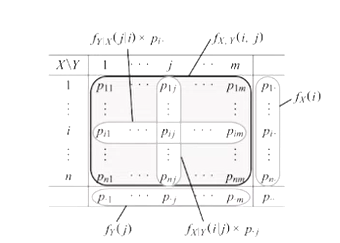
\includegraphics[width=7.0cm]{D_9/img_1.png}
\caption{2次元離散型確率変数の分布}
\end{center}
\end{figure}
\end{document}
%本文ここまで=========================================================
